%-----------------------------------------------------------------
% Modelo de Tese/Dissertação
% Autora: Fabiana Frata Furlan Peres 
% 2014 
%-----------------------------------------------------------------
%% ADAPTADO DE:
%% modelo de Documento TCC da Unioeste   
%%
%% que por sua vez foi ADAPTADO DE: 
%% abtex2-modelo-trabalho-academico.tex, v-1.6 laurocesar
%% Copyright 2012-2013 by abnTeX2 group at http://abntex2.googlecode.com/ 
% ------------------------------------------------------------------------
% abnTeX2: Modelo de Trabalho Academico (tese de doutorado, dissertacao de
% mestrado e trabalhos monograficos em geral) em conformidade com 
% ABNT NBR 14724:2011: Informacao e documentacao - Trabalhos academicos - Apresentacao
%
% ------------------------------------------------------------------------
%DECLARAÇÃO DO TIPO DE DOCUMENTO, TAMANHO DA FOLHA E FONTE
%-----------------------------------------------------------------
\documentclass[12pt,oneside,a4paper,english,french,spanish]{abntex2}

%-----------------------------------------------------------------
%DEFINIÇÃO DOS PACOTES UTILIZADOS
%-----------------------------------------------------------------
\usepackage{cmap}				% Mapear caracteres especiais no PDF
\usepackage{lmodern}			% Usa a fonte Latin Modern			
\usepackage[T1]{fontenc}		% Selecao de codigos de fonte.
\usepackage[utf8]{inputenc}		% Codificacao do documento (conversão automática dos acentos)
\usepackage{lastpage}			% Usado pela Ficha catalográfica
\usepackage{indentfirst}		% Indenta o primeiro parágrafo de cada seção.
\usepackage{color}				% Controle das cores
\usepackage{graphicx}			% Inclusão de gráficos

\usepackage{lipsum}			

\usepackage{amsmath}
\usepackage{amssymb}

% Fonte "Arial"
\usepackage{helvet}
\renewcommand{\familydefault}{\sfdefault}

% Pacotes de citações
\usepackage[alf,abnt-emphasize=bf,bibjustif]{abntex2cite}	% Citações padrão ABNT
% ------------------------
% CONFIGURAÇÕES DA APARENCIA DO PDF FINAL
% ------------------------ 
\definecolor{blue}{RGB}{41,5,195}% alterando o aspecto da cor azul
% informações do PDF
\makeatletter
\hypersetup{     	
		pdftitle={\@title}, 
		pdfauthor={\@author},
    	pdfsubject={\imprimirpreambulo},
	    pdfcreator={LaTeX with abnTeX2},
		pdfkeywords={abnt}{latex}{abntex}{abntex2}{trabalho acadêmico}, 
		colorlinks=true,       		% false: boxed links; true: colored links
    	linkcolor=black,          	% color of internal links
    	citecolor=black,        		% color of links to bibliography
    	filecolor=magenta,      		% color of file links
		urlcolor=blue,
		bookmarksdepth=4
}
\makeatother

%-------------------------------------------------------
%coloque aqui as informações referentes a sua dissertação/tese
%-------------------------------------------------------
\titulo{ESTUDO SOBRE SEGURANÇA EM REDE DE COMPUTADORES DOMÉSTICAS UTILIZANDO PROTOCOLOS DE SEGURANÇA}
\autor{LEANDRO SOLAGNA\\MATHEUS FELIPE BONETTI CASTEGNARO}
\orientador{Prof. Esp. João Paulo de Lima Barbosa}
%\coorientador{}
\local{FOZ DO IGUAÇU}
\data{2016}
\preambulo{Trabalho de conclusão de curso apresentado como requisito obrigatório para obtenção do título de Bacharel em Ciência da Computação da Faculdade Anglo-Americano de Foz do Iguaçu.} % DADOS para CAPA e FOLHA DE ROSTO


%----------------------------------------------------------------- 
% CAPA
\renewcommand{\imprimircapa}{%
  \begin{capa}
  	\begin{center} %Isso eu fiz
  		\large{FACULDADE ANGLO-AMERICANO DE FOZ DO IGUAÇU}
  	\end{center}
    \center
    %{\imprimirautor} %Dica da Tássia
        
    %{\ABNTEXchapterfont\large\imprimirautor} %Original
    {\ABNTEXchapterfont\imprimirautor} %Isso eu fiz

    \vspace*{8cm}
    %{\imprimirtitulo} Dica da Tássia
    \ABNTEXchapterfont\bfseries\large\imprimirtitulo
    \vfill
    
    \large\imprimirlocal

    \large\imprimirdata
    
    \vspace*{1cm}
  \end{capa}
}

\makeatletter
%----------------------------------------------------------------- 
% FOLHA DE ROSTO
\renewcommand{\folhaderostocontent}{
		\center	
		%{\large\textbf\imprimirautor} %Original
			{\large\imprimirautor} %Eu fiz
	
	    \vspace*{8cm}		
		
		
		{\large\textbf\imprimirtitulo}
	
		\vspace*{3cm}	

		\abntex@ifnotempty{\imprimirpreambulo}{
			\hspace{.3\textwidth}
			\begin{minipage}{.55\textwidth}
			
				\SingleSpacing
				\imprimirpreambulo				
				\SingleSpacing				
				{\imprimirorientadorRotulo~\imprimirorientador\par}
				\SingleSpacing	
		        \abntex@ifnotempty{\imprimircoorientador}{
		             {\imprimircoorientadorRotulo~\imprimircoorientador}
		}
		\end{minipage}
		
			\vspace*{\fill}
		}
		
		
		{\large\textbf\imprimirlocal}
		
		{\large\textbf\imprimirdata}		
}

%****************************************************
%outras configurações 
%***********************************************************
\setlength{\parindent}{1.3cm} % Tamanho do parágrafo
\setlength{\parskip}{0.2cm}  % Controle do espaçamento entre um parágrafo e outro
	% Altera o tamanho das fontes dos capítulos e dos apêndices
\renewcommand{\ABNTEXchapterfont}{\bfseries}
\renewcommand{\ABNTEXchapterfontsize}{\large}
\renewcommand{\ABNTEXsectionfontsize}{\normalfont}

% Separação de Palavras:
%\hyphenation{}
\hyphenation{teorias}
\hyphenation{baseados}
\hyphenation{MATLAB}
\hyphenation{Pyramid}
\hyphenation{Mar-cação}
\hyphenation{lin-guagem}
\hyphenation{matplotlib}
\hyphenation{sociali-zação}
\hyphenation{bi-bli-oteca}
\hyphenation{Notebook}
\hyphenation{profis-si-onais}
\hyphenation{ar-quivos}
\hyphenation{usu-ário}
\hyphenation{LinkedIn}

	% Configura layout para elementos textuais

\makepagestyle{abnt_ufpr}

\makeoddhead{abntchapfirst}{}{}{\ABNTEXfontereduzida\thepage}

\pagestyle{abnt_ufpr}



\newtheorem{theorem}{Teorema}[chapter]
\newtheorem{definition}[theorem]{Defini\c{c}\~{a}o}
\newtheorem{proposition}[theorem]{Proposi\c{c}\~{a}o}

\makeatother
%********************************************************************
%*********************************************************************
% Essa parte para baixo até o fim foi tudo copiado da TASSIA

%\newcommand{\quadroname}{Quadro}
%\newcommand{\listofquadrosname}{Lista de quadros}

%\newfloat[chapter]{quadro}{loq}{\quadroname}
%\newlistof{listofquadros}{loq}{\listofquadrosname}
%\newlistentry{quadro}{loq}{0}

% configurações para atender às regras da ABNT
%\counterwithout{quadro}{chapter}
%\renewcommand{\cftquadroname}{\quadroname\space}
%\renewcommand*{\cftquadroaftersnum}{\hfill--\hfill}

%****************************************************
%outras configurações
%***********************************************************
%\setlength{\parindent}{1.3cm} % Tamanho do parágrafo
%\setlength{\parskip}{0.0cm}  % Controle do espaçamento entre um parágrafo e outro

% Altera o tamanho das fontes dos capítulos e dos apêndices

\renewcommand{\ABNTEXchapterfont}{\normalfont\fontseries{b}\selectfont}
\renewcommand{\ABNTEXchapterfontsize}{\normalsize}
\renewcommand{\ABNTEXpartfont}{\fontseries{b}\selectfont\selectfont}
\renewcommand{\ABNTEXpartfontsize}{\normalsize}
\renewcommand{\ABNTEXsectionfont}{\normalfont\selectfont}
\renewcommand{\ABNTEXsectionfontsize}{\normalsize}
\renewcommand{\ABNTEXsubsectionfont}{\normalfont\selectfont}
\renewcommand{\ABNTEXsubsectionfontsize}{\normalsize}
\renewcommand{\ABNTEXsubsubsectionfont}{\normalfont\selectfont}
\renewcommand{\ABNTEXsubsubsectionfontsize}{\normalsize}
\renewcommand{\ABNTEXsubsubsubsectionfont}{\normalfont\itshape\selectfont}
\renewcommand{\ABNTEXsubsubsubsectionfontsize}{\normalsize}


% CONFIGURACAO DO SUMARIO

% Sumário
\renewcommand*{\cftsectionfont}{\normalfont}
\renewcommand*{\cftsubsubsectionfont}{\normalfont}
\renewcommand*{\cftsubsectionfont}{\normalfont}
\renewcommand*{\cftparagraphfont}{\normalfont\itshape}

% -----------------------------------------------------------------------------
% Modifica o espaçamento no sumário
% Nao ha espacos, para as entradas de capitulos
\setlength{\cftbeforeparagraphskip}{0pt}
\setlength{\cftbeforesubsectionskip}{0pt}
\setlength{\cftbeforesectionskip}{0pt}
\setlength{\cftbeforesubsubsectionskip}{0pt}
\setlength{\cftbeforechapterskip}{0pt}



\addto\captionsbrazil{
	\renewcommand{\bibname}{REFER\^ENCIAS}
}

\addto\captionsbrazil{\renewcommand{\listadesiglasname}{LISTA DE ABREVIATURAS}}
\addto\captionsbrazil{\renewcommand{\listfigurename}{LISTA DE ILUSTRAÇÕES}}
\addto\captionsbrazil{\renewcommand{\listtablename}{LISTA DE TABELAS}}
\addto\captionsbrazil{\renewcommand{\contentsname}{SUMÁRIO}}
\addto\captionsbrazil{\renewcommand\appendixtocname{APÊNDICES}\renewcommand\appendixpagename{APÊNDICES}}
\addto\captionsbrazil{\renewcommand{\figurename}{FIGURA}}
\addto\captionsbrazil{\renewcommand{\tablename}{TABELA}}


% Configura layout para elementos textuais

%\makepagestyle{abnt_ufpr}


%\makeoddhead{abntchapfirst}{}{}{\ABNTEXfontereduzida\thepage}

%\pagestyle{abnt_ufpr}

%%%%%%%% AMBIENTES %%%%%%%%%%
%\newtheorem{teo}{Teorema}[chapter]
%\newtheorem{cor}[teo]{Corol\'{a}rio}
%\newtheorem{lem}[teo]{Lema}
%\newtheorem{prop}[teo]{Proposi\c{c}\~{a}o}
%\newtheorem{defn}[teo]{Defini\c{c}\~{a}o}
%\newtheorem{Ex}[teo]{Exemplo}
%\newtheorem{obs}[teo]{Observa\c{c}\~{a}o}
%\newtheorem{prob}[teo]{Problema}
%\newtheorem{conc}[teo]{Conclusão}
%\newenvironment{dem}{\smallskip \noindent{\bf Demonstra\c{c}\~{a}o}: }
%{\hfill $\Box$\hspace{0in}\medskip}

%%%%%%%% COMANDOS FRECUENTES %%%%%%%%
%\newcommand{\eq}{\begin{equation}}
%	\newcommand{\ee}{\end{equation}}
%\newcommand{\R}{{\mathbb R}}
%\newcommand{\N}{{\mathbb N}}
%\newcommand{\K}{{\mathbb K}}
%\newcommand{\Q}{{\mathbb Q}}
%\newcommand{\Z}{{\mathbb Z}}
%\newcommand{\V}{{\mathbb V}}
%\newcommand{\D}{{\mathcal{D}}}
%\newcommand{\C}{{\mathbb C}}
%\newcommand{\di} {\displaystyle}
%\newcommand{\I}{{\displaystyle\int_{0}^{T} \displaystyle\int_{0}^1 }}
%\newcommand{\Ia}{{\displaystyle\int_{0}^{1} \displaystyle\int_{0}^T }}
%\newcommand{\Ii}{{\displaystyle\int_{0}^{t} \displaystyle\int_{0}^1 }}
%\newcommand{\Ib}{{\displaystyle\int_{0}^{1} \displaystyle\int_{0}^t }}
%%%%%%%%%%%%%%%%%%%%%%%%%%%
%\makeatother % Configurações DO DOCUMENTO

\makeindex
% ------------------------
% Início do documento
% ------------------------ 
\begin{document}
\frenchspacing % Retira espaço extra obsoleto entre as frases.

% ----------------------------------------------------------
% ELEMENTOS PRÉ-TEXTUAIS
% ----------------------------------------------------------
\imprimircapa
\imprimirfolhaderosto* % (o * indica que haverá a ficha bibliográfica)

%\begin{fichacatalografica}

	\vspace*{15cm}       %  Posição  vertical

	\hrule %  Linha  horizontal

	\begin{center}       %  Minipage  Centralizado

	\begin{minipage}[c]{12.5cm}  %  Largura
	
	SobreNome, Nome1 Nome2 % Nome de referência. Por ex. Silva, João Paulo
 
	\hspace{0.5cm}  \imprimirtitulo~/~\imprimirautor~--~\imprimirlocal,  \imprimirdata.
	
	\hspace{0.5cm}  \pageref{LastPage}  p.  :  il.\\

	\hspace{0.5cm}  \imprimirorientadorRotulo ~\imprimirorientador\\

	\hspace{0.5cm}

\parbox[t]{\textwidth}{\imprimirtipotrabalho ~--~ Universidade Estadual do Oeste do Paraná (UNIOESTE). Centro de Engenharias e Ciências Exatas (CECE). Curso de Ciência da Computação, \imprimirdata.}\\

\hspace{0.5cm}
	1.  Palavra-chave1.
	2.  Palavra-chave2.
	I.  Orientador.
	II.  Universidade Estadual do Oeste do Paraná (UNIOESTE).
	III. Centro de Engenharias e Ciências Exatas (CECE).
	IV. Curso de Ciência da Computação.
	V.  \imprimirtitulo\\
	
	\hspace{8.75cm}  CDU  02:141:005.7\\

	\end{minipage}
	\end{center}
	\hrule
\end{fichacatalografica}

%\begin{folhadeaprovacao} %[TERMO DE APROVAÇÃO]
\begin{center}
	\vspace*{1cm}  
  	\large\textbf{TERMO DE APROVAÇÃO}
  	
  	\vspace*{1cm} %minha mudança
  	%\vspace*{2cm}
  	{\large\textbf\imprimirautor}

   \vspace*{1cm} %minha modif
   %\vspace*{2cm}
    {\large\textbf\imprimirtitulo}   
 \end{center}     
  
	
	\hspace{.4\textwidth}
	\SingleSpace\noindent\normalsize{Trabalho de conclusão de curso apresentado como requisito obrigatório para obtenção do título de Bacharel em Ciência da Computação da Faculdade Anglo-Americano de Foz do Iguaçu, pela seguinte banca examinadora:}
%	\noindent\paragraph
   
 %  \end{center}
    
  
   %\vspace*{1.5cm}
   \vspace*{0.5cm}  %minha modif
   \assinatura{{\imprimirorientador}\\Faculdade Anglo-Americano\\(Orientador)}
   \assinatura{Prof. Banca 2\\Faculdade Anglo-Americano}
   \assinatura{Prof. Banca 3\\Faculdade Anglo-Americano} 
   \vspace*{2.5cm}
   \begin{center}
   	%{\imprimirlocal, \ \imprimirdata}
   	{Foz do Iguaçu, 30 de novembro de 2015}
   \end{center}
   
 
\end{folhadeaprovacao}
%\begin{dedicatoria}
   \vspace*{\fill}
   \begin{flushright}
   	\textit{Dedico a....}
   	
   \end{flushright}
\end{dedicatoria}

%% ---
% Agradecimentos
% ---
\begin{agradecimentos}[AGRADECIMENTOS]
Agradeço...

\end{agradecimentos}


% ---
% Epígrafe
% ---
\begin{epigrafe}
    \vspace*{\fill}
	\begin{flushright}
		\textit{"Eu enfrento leões.\\ Nado com os tubarões.\\ Se por ventura cair, já estou de pé.
		(Drawtheline)}
	\end{flushright}
\end{epigrafe}


\vspace*{-0.65cm}
% resumo em português
\begin{resumo}[RESUMO]	
Esse trabalho tem como objetivo, avaliar se os equipamentos de redes domésticas atuais, possuem suporte aos protocolos SEND e RA Guard. O estudo de caso, apresentará as características de cada protocolo, assim como o seu funcionamento e protocolos que trabalham em conjunto. Demonstrando também, a importância de se ter segurança mesmo que a rede de computadores seja pequena.


 \vspace{\onelineskip}
    
 \noindent
 \textbf{Palavras-chaves}: SEND, RA Guard, IPv6, Segurança.
 % 4 palavras separadas por . (ponto)
\end{resumo}

\vspace*{-0.65cm}
\begin{resumo}[ABSTRACT]
 \begin{otherlanguage*}{english}
   This project has as a goal, the evaluation of small offices network equipaments when it comes to security. As for that, it will be through SEND and RA Guard protocols, as if these equipaments have any sort of support to these security protocolos. It will also be studied, their characteristics, how they work and other protocols that work together. This study will also show how important is to have network security, even for a small office.
   
   
   \vspace{\onelineskip}
 
   \noindent 
   \textbf{Keywords}: SEND, RA Guard, IPv6, Security.
 \end{otherlanguage*}
\end{resumo}


%\pdfbookmark[0]{\listfigurename}{lof}% inserir lista de ilustrações
%\listoffigures*
%\cleardoublepage

%\pdfbookmark[0]{\listtablename}{lot}% inserir lista de tabelas
%\listoftables*
%\cleardoublepage


\begin{siglas}

	\item[UCLA]     \textit{University of California, Los Angeles} - Universidade da Califórnia, Los Angeles\footnote{Tradução dos autores}
	\item[SIR]      \textit{Stanford Research Institute} - Instituto de Pesquisa \textit{Stanford}\footnotemark[1]
	\item[IP]       \textit{Internet Protocol} - Protocolo de Internet\footnotemark[1]
	\item[IPv4]     \textit{Internet Protocol version 4} - Protocolo de Internet versão 4\footnotemark[1]
	\item[CIDR]     \textit{Classless Inter-Domain Routing} - Roteamento Intra Domínio Sem Classe\footnotemark[1]
	\item[NAT]      \textit{Network Address Translation} - Tradução de Endereço de Rede\footnotemark[1]
	\item[IPv6]     \textit{Internet Protocolo version 6} - Protocolo de Internet versão 6\footnotemark[1]
	\item[ICMP]     \textit{Internet Control Message Protocol} - Protocolo de Controle de Mensagem da Internet\footnotemark[1]
	\item[DHCP]     \textit{Dynamic Host Configuration Protocol} - Protocolo de Configuração Dinâmica de Host\footnotemark[1]
	\item[IPSec]    \textit{IP Security Protocol} - Protocolo de Segurança\footnotemark[1]
	\item[ARP]      \textit{Address Resolution Protocol} - Protocolo de Resolução de Endereço\footnotemark[1]
	\item[RARP]     \textit{Reverse Address Resolution Protocol} - Protocolo de Resolução Reversa de Endereços\footnotemark[1]
	\item[IGMP]     \textit{Internet Group Management Protocol} - Protocolo Gerenciamento de Grupos da Internet\footnotemark[1]
	\item[ICMPv6]   \textit{Internet Control Message Protocol version 6} - Protocolo de Controle de Mensagem da Internet versão 6\footnotemark[1]
	\item[RS]       \textit{Router Solicitation}
	\item[RA]       \textit{Router Advertisement}
	\item[NA]       \textit{Neighbor Solicitation}
	\item[NS]       \textit{Neighbor Advertisement}
	\item[MAC]      \textit{Media Access Control} - Controle de Acesso à Mídia\footnotemark[1]
	\item[NDP]      \textit{Neighbor Discovery Protocol} - Protocolo de Descoberta de Vizinhança\footnotemark[1]
	\item[SEND]     \textit{SEcure Neighbor Discovery}
	\item[RA Guard] \textit{Router Advertisement Guard}

%fim das siglas do capitulo 1
%--------------------------------------------------------------------------------------------------
%--------------------------------------------------------------------------------------------------
%começo das siglas do capitulo 2

	\item[DARPA]    \textit{Defense Advanced Research Projects Agency}
	\item[ARPANET]  \textit{Advanced Research Projects Agency Network}
	\item[OSI]      \textit{Open System Interconnection model}
	\item[TCP]      \textit{Transmission Control Protocol}
	\item[NAT]      \textit{Network Address Translation}
	\item[IANA]     \textit{Internet Assigned Numbers Authority}
	\item[ICAN]     \textit{Internet Corporation for Assigned Names and Numbers}
	\item[RIR]      \textit{Regional Internet Registries} - Registro Regional da Internet
	\item[LACNIC]   \textit{Latin America and Caribbean Network Information} - Registro de Endereçamento da Internet para América Latina e Caribe
	\item[]      \textit{}
%fim das siglas do capitulo 2
%--------------------------------------------------------------------------------------------------
%--------------------------------------------------------------------------------------------------
%começo das siglas do capitulo 3

\end{siglas}
  % inserir lista de abreviaturas e siglas

%\begin{simbolos}
  \item[$ \Gamma $] Letra grega Gama
  \item[$ \Lambda $] Lambda
  \item[$ \zeta $] Letra grega minúscula zeta
  \item[$ \in $] Pertence
\end{simbolos}
% inserir lista de símbolos

\vspace*{0cm}
\pdfbookmark[0]{\contentsname}{toc}% inserir o sumario
\tableofcontents*
\cleardoublepage


% ----------------------------------------------------------
% ELEMENTOS TEXTUAIS
% ----------------------------------------------------------
\textual

\chapter{INTRODUÇÃO}\label{ch:introducao}

O crescimento contínuo e global da Internet é um dos fenômenos mais interessantes e excitantes em redes. Há algumas décadas, não se imaginava que um projeto de pesquisa envolvendo duas universidades da Califórnia – UCLA (Universidade da Califórnia, Los Angeles) e SRI (Instituto de Pesquisa Stanford), se tornaria o principal meio de comunicação no dia a dia das pessoas.

Para que essa comunicação aconteça, protocolos que ditam as regras de conexão, entre uma origem e destino, foram criados. Ou seja, possibilitando assim a comunicação entre pessoas ou máquinas, não importando a sua localização global. Entre vários protocolos que foram criados, o mais importante foi, o IP (Protocolo de Internet). O IP é responsável por dar um endereço único para cada dispositivo conectado em uma rede de computadores, permitindo assim, que as informações cheguem ao seu destino. citar: http://www.infowester.com/ip.php

A partir de 1983, a Internet começou a usar o IP versão 4 (IPv4). Isto fez com que a rede mundial de computadores crescesse em um ritmo acelerado, com vários equipamentos sendo criados e necessitando de um endereço único para funcionar normalmente. Por causa disso, cientistas e especialistas perceberam no final da década de 80, que os números de IPv4 estavam próximos de esgotarem. citar: http://ipv6.br/post/ipv6-um-desafio-tecnico-para-a-internet/

Dessa forma, começaram pesquisas para se encontrar uma solução adequada para esse problema. Nos anos 90, solução como o CIDR (Roteamento Intra Domínio Sem Classe) foi proposto, com o intuito de usar os endereços IPs de forma mais eficiente. Em tempos mais recentes, começo dos anos 2000, o NAT (Tradução de Endereço de Rede) foi proposto, mascarando IPs inválidos para que os usuários possam acessar a nuvem. Obviamente, essas soluções só foram propostas como temporárias, o grande problema ainda existia, o limite de endereços IPv4.
A solução proposta foi a atualização do protocolo, usado na época, para um outro que pudesse gerar mais endereços únicos. Foi então desenvolvido o IP versão 6 (IPv6). Nessa versão, a característica principal foi o aumento de número de endereços, passando de 4 bilhões para mais de 340 undecilhões. citar: http://ipv6.br/post/enderecamento/

Os cientistas aproveitaram essa oportunidade para mudar outras características do protocolo, algumas dessas foi a alteração do cabeçalho para um menos complexo de se entender, protocolos que auxiliam o IPv6 no seu funcionamento, ICMP (Protocolo de Controle de Mensagem da Internet), DHCP (Protocolo de Configuração Dinâmica de Host) e IPSec (Protocolo de Segurança) também foram modificados.

Assim como na versão anterior, o IPv6 usa o protocolo de controle de mensagens da Internet ICMP, que tem como responsabilidade enviar mensagens de erro indicando que o serviço, roteador ou um endereço de rede está indisponível. No IPv6, além de reportar erros no processamento de pacotes, realizar diagnósticos e enviar mensagens sobre as características da rede, o protocolo ICMPv6 assumiu também funcionalidades dos protocolos ARP (Protocolo de Resolução de Endereço), RARP (Protocolo de Resolução Reversa de Endereços) e IGMP (Protocolo Gerenciamento de Grupos da Internet). citar: http://www.teleco.com.br/tutoriais/tutorialredeipmig1/pagina_2.asp

Os protocolos ARP e RARP, em geral, são utilizados para encontrar um endereço único em um dispositivo em uma rede. O protocolo IGMP tem como função controlar os membros de um grupo de \textit{multicast}.

Com o ICMPv6 (Protocolo de Controle de Mensagem da Internet versão 6), várias mensagens são trocadas em uma rede local, sendo quatro delas fundamentais para a descoberta de hosts IPv6 vizinhos:

\begin{itemize}
\item RS (\textit{Router Solicitation}): mensagem enviada de uma estação que deseja aprender informações de um roteador de uma rede local;
\item RA (\textit{Router Advertisement}): mensagens enviadas em respostas às mensagens RS, podendo também ser usada para enviar anúncios não solicitados para toda a rede, informando da sua existência;
\item NS (\textit{Neighbor Solicitation}): mensagem enviada por uma máquina com o objetivo de encontrar o endereço MAC (Controle de Acesso à Mídia) de um endereço IPv6;
\item NA (\textit{Neighbor Advertisement}): São respostas à mensagens NS ou para informar a mudança de endereço de uma máquina.
\end{itemize}

Com o protocolo ICMP atualizado, um novo protocolo dependente do ICMP foi criado, o NDP(Protocolo Descoberta de Vizinhança). O NDP do ICMPv6 permite saber quais são as máquinas da rede, encontrar roteadores vizinhos, detectar endereços duplicados e detectar outras anomalias que possam acontecer dentro de uma rede de computadores. citar: https://tools.ietf.org/html/rfc4861

O protocolo IPv6 ainda é considerado um protocolo novo, por isso, suas vulnerabilidades ainda não foram exploradas ao máximo. citar: https://securityintelligence.com/the-importance-of-ipv6-and-the-internet-of-things/

Assim como no seu antecessor (IPv4), o IPv6 possui vulnerabilidades que podem ser exploradas através de ataque como \textit{man-in-the-middle}, cujo objetivo é o roubo de informações ou ataques que possam negar algum serviço, fazendo com que o usuário da rede não consiga utilizá-la.

Para fornecer segurança contra ataques que possam se passar por uma máquina ou um dispositivo da rede foi criado uma extensão do protocolo NDP, chamado de SEND (\textit{SEcure Neighbor Discovery}). Este protocolo propõe solução aos seguintes itens: citar: https://tools.ietf.org/html/rfc3971

\begin{itemize}
\item Criação de uma cadeia de certificados;
\item A utilização de endereços gerados criptograficamente;
\item Criação de opções para proteger todas as mensagens relativas ao NDP;
\item Prevenir ataques de reenvio de mensagens por meio de duas novas opções no NDP;
\end{itemize}

Quando se usa o IPv6, sem o apoio do SEND em todos os dispositivos da rede, há sempre o risco de lidar com problemas que envolvem o envio indevido dos RA, que são mensagens enviadas por roteadores em resposta às mensagens de requisitos ou RS, por roteadores não autorizados ou indevidamente configurados na rede. citar: http://www.teleco.com.br/tutoriais/tutorialredeipmig1/pagina_2.asp

Uma alternativa para esse problema é o protocolo RA Guard (\textit{Router Advertisement Guard}), que surgiu devido à dificuldade de implementação do SEND.

O IPv6 RA Guard monitora mensagens de RA originadas de um roteador não autorizado. Esse protocolo analisa as RA e filtra as mensagens de dispositivos não autorizados, através de uma tabela, que possui as informações dos roteadores autorizados na rede. citar: https://tools.ietf.org/html/rfc6105

Essa técnica é usada para ajudar o administrador a identificar ataques como \textit{man-in-the-middle}, um roteador da rede que não está autorizado e negação de serviço por configuração inválida. https://community.infoblox.com/t5/IPv6-Center-of-Excellence/Why-You-Must-Use-ICMPv6-Router-Advertisements-RAs/ba-p/3416


\section{JUSTIFICATIVA}\label{sec:justificativa}

Atualmente, existem métodos com o objetivo de roubar informações. Alguns destes métodos podem ser utilizados para, ao infiltrar-se, se passar por um roteador ou uma máquina na rede, visando ter o tráfego da rede passando por eles, dessa forma, obtêm-se pacotes contendo informações sigilosas.

Com o intuito de evitar esses possíveis ataques, os protocolos SEND e RA Guard foram criados para que uma ação e um alerta ocorram no momento em que se detecta uma invasão dentro de uma rede.

Nos dias atuais, é necessário saber se os dispositivos de redes domésticas vendidos no mercado suportam no mínimo um desses protocolos. 

\section{OBJETIVOS}\label{sec:objetivos}

Nesta sessão serão abordados os objetivos gerais e específicos deste trabalho. Apresentando os pontos de interesse, no qual almeja-se chegar ao fim do projeto aqui apresentado.

\subsection{Objetivo Geral}

Descobrir quais atuais equipamentos de uma rede de porte pequeno, possuem suporte aos protocolos de segurança SEND e RA Guard. Para isso, haverá a necessidade de implementar esses protocolos e testá-los nos equipamentos instalados. Por fim, uma tabela com os dispositivos testados será apresentado, nela, constará os resultados obtidos durante os testes.

\subsection{Objetivos Específicos}\label{subsec:objetivos_especificos}

\begin{itemize}
\item Pesquisar sobre os funcionamentos dos protocolos SEND e RA Guard, assim como os protocolos de IPv6 que trabalham junto a eles.
\item Montar um ambiente de testes, com equipamentos atuais, para que os protocolos pesquisados possam ser colocados em prática.
\item Inserir os protocolos de proteção no ambiente de testes, para que possam ser demonstrados.
\item Através de uma tabela comparativa, apresentar quais os dispositivos atuais que possuem suporte para as técnicas de proteção abordadas.
\end{itemize}

\section{ORGANIZAÇÃO DO TRABALHO}\label{sec:organizacao-trabalho}

Esta sessão, apresentará uma breve descrição dos capítulos presentes neste trabalho.
No capítulo 2, serão descritos os fundamentos teóricos, com a finalidade de compreender o tema proposto. Temas como funcionalidades do IPv4, IPv6, segurança, ameaças e vulnerabilidades serão mostrados

No capítulo 3, são apresentados os protocolos de segurança SEND e RA Guard. E abordado a sua funcionalidade e seus componentes.

No capítulo 4, apresentam-se as formas de implementações, equipamentos necessários para isso, equipamentos das quais serão testados e definições necessárias para o entendimento acerca do tema abordado neste trabalho.

No capítulo 5, apresentam-se os resultados obtidos com o desenvolvimento do projeto de forma geral.

No capítulo 6, a conclusão e trabalhos futuros são abordados.


% ------------------------
% Capítulos da Monografia
% ------------------------
\chapter{REVISÃO BIBLIOGRÁFICA}\label{ch:rev-bibs}

O inicio das redes de computadores aconteceu nos Estados Unidos, onde pesquisadores do DARPA (\textit{Defense Advanced Research Projects Agency}) começaram a experimentar comunicações entre computadores com o objetivo de conectar os departamentos de pesquisas com as bases miliares Americanas. Mas, como os estados unidos estavam plena guerra fria e toda comunicação das redes passavam por um computador central que se encontravam no Pentágono sua comunicação era extremamente vulnerável. Bastava apenas a antiga URSS atacar o Pentágono que toda a conexão Americana era afetada(Refe: <http://www.inf.furb.br/~pericas/orientacoes/EstudoIPv62006.pdf>)

E com isso surgiu a ARPANET (\textit{Advanced Research Projects Agency Network}), com um Back Bone por baixo da terra que ligava os militares aos pesquisadores, tendo como primeiro nó a UCLA e o segundo nó a SRI, onde receberam a primeira mensagem de nó-a-nó \cite{comeco-internet}.

Isso tudo levou a adição de vários outros nós à rede. Infelizmente, os problemas começaram a surgir, ficando claro que seria necessário desenvolver protocolos para maior garantia de comunicação entre todos os nós, e, em razão disso, protocolos como o IPv4 foram desenvolvidos.

Com o esgotamento do número endereços IPv4 mais próximo a cada dia, tecnologias começaram a ser desenvolvidas para o IPv6. Iniciando assim, pesquisas para extensões deste protocolo, criação de novos protocolos de segurança e maior aplicação em tecnologias que utilizam IPv6.

Dentro de várias pesquisas, surgiram duas para segurança em redes que utilizam o IPv6, das quais deram inspirações nesse trabalho. Cujo foco é saber se equipamentos de redes domésticas possuem suporte para protocolos de segurança em rede.

Não é possível falar de IPv6 e suas tecnologias, sem mencionar o seu antecessor IPv4.

\section{IPv4}\label{sec:protIPv4}

A primeira versão do protocolo de Internet a ser utilizada globalmente. Trabalha na camada de rede do modelo OSI (\textit{Open System Interconnection model}) e na camada de Internet no modelo TCP (\textit{Transmission Control Protocol})/IP.

Responsável por identificar hospedeiros onde providencia um endereço único para cada hospedeiro em uma rede. O cabeçalho deste protocolo contem 14 campos, da qual cada um possui a sua obrigação.

Com suporte a três tipos diferentes de modos de endereçamento, da qual se chamam \textit{unicast}, \textit{broadcast} e \textit{multicast}.

<<<<<<< HEAD
O protocolo divide cada endereço em uma hierarquia de dois níveis, prefixo e sufixo, o prefixo de um endereço identifica a rede a qual o dispositivo se liga, e o sufixo identifica um dispositivo específico na rede. Um endereço de IP é um número de 32 \textit{bits}. No início, o endereço pertencia a uma de cinco classes, em que a classe de um endereço era determinada pelo valor dos quatro primeiros bits, onde a uma rede física que contivesse entre 257 e 65.536 hospedeiros era atribuído o valor de prefixo B. As redes menores era atribuído um valor prefixo de classe C, e as redes maiores era atribuído o prefixo de classe A. (Refe: Livro do joão, usado nas aulas de redes)
=======
O protocolo divide cada endereço em uma hierarquia de dois níveis, prefixo e sufixo, o prefixo de um endereço identifica a rede a qual o dispositivo se liga, e o sufixo identifica um dispositivo específico na rede. 
>>>>>>> c27b5094154337ec47832a3f9dff961d1ca9bb2b

Um endereço de IP é um número de 32 bits. No início, o endereço pertencia a uma de cinco classes, em que a classe de um endereço era determinada pelo valor dos quatro primeiros bits, onde a uma rede física que contivesse entre 257 e 65.536 hospedeiros era atribuído o valor de prefixo B. As redes menores era atribuído um valor prefixo de classe C, e as redes maiores era atribuído o prefixo de classe A. (Refe: Livro do joão, usado nas aulas de redes)

Apesar disso, existem endereços reservados para uso pessoal. Toda a classe de IP's possui endereços reservados que podem ser utilizados em uma rede local, por exemplo, em empresas e em casas. Esses endereços podem ser chamados de IPv4 inválidos, pois não são roteáveis na Internet.

Em razão disso foi desenvolvido a tecnologia NAT (\textit{Network Address Translation}), que faz a tradução de um IP inválido para IP válido. Basicamente o NAT  pega o seu endereço inválido e o mascara utilizando o único IP válido que a pessoa possui. Dessa forma, a rede externa acredita que o usuário está utilizando aquele IP válido para acessar páginas \textit{web}.

Para receber um endereço IP, o computador procura um servidor DHCP, se houver um na rede, um endereço é atribuído. Outra alternativa é configurar manualmente um endereço IP para que então o computador possa se comunicar com outros na rede.

A alocação de IPv4 é globalmente gerenciada pela IANA (\textit{Internet Assigned Numbers Authority}) em coordenação com a ICANN (\textit{Internet Corporation for Assigned Names and Numbers}). A IANA trabalha junto com os cincos RIRs (Registro Regional da Internet) existentes das quais são orgões que gerenciam a distribuição de IPv4 e IPv6. Na américa latina o orgão responsável por entrega de endereços IPv4 válidos é a LACNIC (Registro de Endereçamento da Internet para América Latina e Caribe).

<<<<<<< HEAD
Como mencionado anteriormente, os endereços dessa versão estavam próximos de esgotarem e se isso ocorresse, a rede mundial teria vários problemas, mesmo com tecnologias surgindo para evitar que isso ocorra, por exemplo NAT. Por essa razão, pesquisas para desenvolver um novo protocolo começaram a ser realizadas, o que fez que surgisse o IPv6 para evitar o esgotamento de IP's espalhados pelo mundo.

\section{As diferenças entre os protocolos}\label{sec:protIPv6}

A principal diferença entre os dois protocolos é o número de bits que mude de apenas 32 \textit{bits} para 128 \textit{bits}, permitindo assim uma mudança radical na atribuição e gerenciamento de endereços IP \cite{}.

Além da diferença principal, houve uma grande 
=======
\section{IPv6}\label{sec:protIPv6}

Com a explosão da internet e com o constante surgimento de tecnologias, aplicações, serviços e dispositivos conectados a rede, os endereços atuais de IPv4 se tornariam escassos. 

Citar - "Foi quando em Junho de 1994, a comissão do IPng (Internet Protocol next generation) revisou todas as propostas e publicou sua recomendação. Sugeriu o SIPP como a base para o novo protocolo IP. O novo protocolo teria endereços de 128 bits e se chamaria IPv6. O número 5 havia sido alocado ao protocolo ST (stream), um protocolo experimental para suportar serviços em tempo real em paralelo com o IP. (NUNES, 2006, internet)."

O novo protocolo atendia as necessidades das empresas em questão de redes com arquiteturas mais escaláveis, com maior segurança e integridade de dados 
>>>>>>> c27b5094154337ec47832a3f9dff961d1ca9bb2b

%\chapter{FUNDAMENTAÇÃO TEÓRICA}\label{ch:fundaments-teorico}
A mineração de dados é um assunto totalmente interdisciplinar podendo ser definido de diversas maneiras. Até mesmo o termo \textit{data mining} não representa realmente todos os componentes desta área. \citeonline{han} exemplificam esta questão comentando sobre a mineração de ouro através da extração de rocha e areia, que é chamado de mineração de ouro e não mineração de rochas ou mineração de areia. Analogamente, a mineração de dados deveria se chamar "mineração de conhecimento através de dados", que infelizmente é um termo um tanto longo. Entretanto, uma referência mais curta, como "mineração de conhecimento", pode não enfatizar a mineração de uma enorme quantidade de dados. Apesar disso, a mineração é um termo que caracteriza o processo de encontrar uma pequena quantia de uma preciosa pepita em uma grande quantidade de matéria bruta. Nesse sentido, um termo impróprio contendo ambos \textit{"data"} e \textit{"mining"} se tornou popular e, como consequência, muitos outros nomes similares surgiram: \textit{knowledge mining from data}, \textit{knowledge extraction}, \textit{data/pattern analysis}, \textit{data archaeology} e \textit{data dredging}.

Na Seção~\ref{sec:kdd} será abordado os conceitos de descoberta de conhecimento em base de dados e a sua diferença em relação ao \textit{data mining}. Logo, na Seção~\ref{sec:data-mining}, é apresentado os métodos e a concepção de \textit{data mining}. Alguns desses métodos tem como prática o uso de aprendizado de máquina que será definido na Seção~\ref{sec:machine-learning}. A Seção~\ref{sec:python} irá caracterizar a linguagem de programação Python e qual a sua vantagem em utilizá-la para a mineração de dados.

%%
% KDD
\section{DESCOBERTA DE CONHECIMENTO EM BASE DE DADOS E \textit{DATA MINING}}\label{sec:kdd}
Muitas pessoas tratam a mineração de dados como um sinônimo para outro termo muito popular, descoberta de conhecimento em base de dados (\textit{knowledge discovery from data}) - KDD, enquanto outros referenciam \textit{data mining} como apenas uma etapa no processo de descoberta de conhecimento em base de dados. O processo de KDD é demonstrado através da  Figura~\ref{kdd-fig} como uma sequência interativa e iterativa dos seguintes passos: \\ \\ \\ \\ \\ \\

\begin{figure}
	\centering
	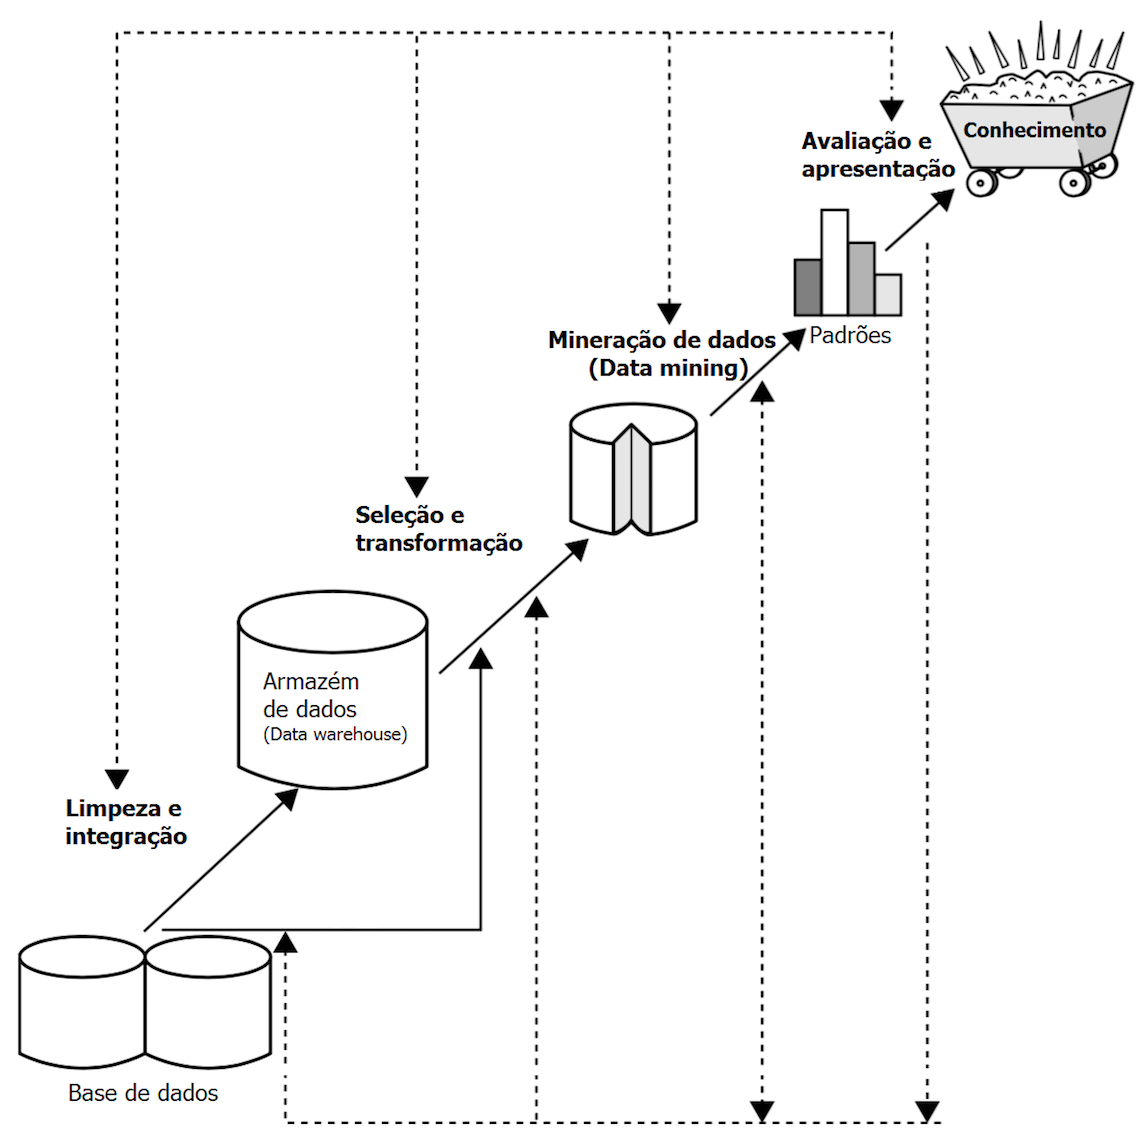
\includegraphics[width=1\textwidth]{Cap3/imagens/kdd}
	\caption{\textsc{Etapas do processo de KDD}}
	\vspace{-0.3cm}
	\legend{\small{FONTE: Adaptado de \citeonline{han}}}
	\label{kdd-fig}
\end{figure}

\begin{enumerate}
	\item \textit{Data cleaning} (Limpeza de dados);
	\item \textit{Data integration} (Integração de dados);
	\item \textit{Data selection} (Seleção de dados);
	\item \textit{Data transformation} (Transformação de dados);
	\item \textit{Data mining} (Mineração de dados);
	\item \textit{Pattern evaluation} (Avaliação de padrões);
	\item \textit{Knowledge presentation} (Apresentação de conhecimento).
\end{enumerate}


De acordo com \apudonline{brachman}{fayyad2}, as etapas são interativas porque envolvem a cooperação da pessoa responsável pela análise de dados, cujo conhecimento sobre o domínio orientará a execução do processo. Por sua vez, a interação deve-se ao fato de que, com frequência, esse processo não é executado de forma sequencial, mas envolve repetidas seleções de parâmetros e conjuntos de dados, aplicações das técnicas de \textit{data mining} e posterior análise dos resultados obtidos, a fim de refinar os conhecimentos extraídos.

KDD refere-se ao processo global de descobrimento de conhecimento útil em bases de dados. \textit{Data mining} é um passo particular neste processo aplicação de algoritmos específicos para extrair padrões (modelos) de dados. Os passos adicionais no processo KDD, como integração de dados, limpeza de dados, seleção de dados, incorporação de conhecimento anterior apropriado e interpretação formal dos resultados de mineração assegura aquele conhecimento útil que é derivado dos dados. A aplicação cega de métodos de \textit{data mining} pode ser uma atividade perigosa que conduz a descoberta de padrões sem sentido \cite{navega}. 

O KDD evoluiu e continua evoluindo da interseção de pesquisas em campos como bancos de dados, aprendizado de máquinas (\textit{machine learning}), reconhecimento de padrões, estatísticas, inteligência artificial, aquisição de conhecimento para sistemas especialistas, visualização de dados, descoberta científica, recuperação de informação e computação de alto-desempenho. Aplicações de KDD incorporam teorias, algoritmos e métodos de todos estes campos \cite{credito-bancario}.


%%
% Data Mining
\section{\textit{DATA MINING}}\label{sec:data-mining}
Apesar do conceito de \textit{data mining}, na maioria das vezes, ser utilizado pelas indústrias, mídias e centros de pesquisa para se referir ao processo de descoberta de conhecimento considerado em sua globalidade, o termo \textit{data mining} poderá ser usado também para indicar o quinto estágio do KDD, sendo um processo essencial na descoberta e extração de padrões de dados. \citeonline{han}, adotam uma visão mais abrangente para a funcionalidade de mineração de dados: \textit{data mining} é o processo de descoberta de padrões interessantes e conhecimentos de um vasto conjunto de dados. A fonte dos dados pode ser banco de dados, \textit{data warehouses}, a Internet, outros repositórios de informações, ou dados correntes em sistemas dinâmicos.

Uma das definições, talvez, mais importante de \textit{data mining} foi elaborada por \citeonline{fayyad} "...o processo não-trivial de identificar, em dados, padrões válidos, novos, potencialmente úteis e ultimamente compreensíveis".

\textit{Data mining} ou mineração de dados, pode ser entendido, então como o processo de extração de informações, sem conhecimento prévio, de algum conjunto de dados e seu uso para tomada de decisões. A mineração de dados se define através de processos automatizados de captura e análise deste conjunto de dados com a finalidade de extrair algum significado, podendo descrever características do passado, como também para predizer futuras tendências \cite{conceito-data-mining}.

Diversos métodos são usados em \textit{data mining} para encontrar respostas ou extrair conhecimento interessante. Esses podem ser obtidos através dos seguintes métodos:

\begin{itemize}
	\item Classificação: associa ou classifica um item a uma ou várias classes. Os objetivos dessa técnica envolvem a descrição gráfica ou algébrica das características diferenciais das observações de várias populações. A ideia principal é derivar uma regra que possa ser usada para classificar, de forma otimizada, uma nova observação a uma classe já rotulada;
	
	\item Modelos de Relacionamento entre Variáveis: associa um item a uma ou mais variáveis de predição de valores reais, conhecidas como variáveis independentes ou exploratórias. Nesta etapa se destacam algumas técnicas estatísticas como regressão linear simples, múltipla e modelos lineares por transformações, com o objetivo de verificar o relacionamento funcional entre duas variáveis quantitativas, ou seja, constatar se há uma relação funcional entre X e Y;
	
	\item Análise de Agrupamento (\textit{Cluster}): associa um item a uma ou várias classes (ou \textit{clusters}). Os \textit{clusters} são definidos por meio do agrupamento de dados baseados em modelos probabilísticos ou medidas de similaridade. Analisar \textit{clusters} é uma técnica com o objetivo de detectar a existência de diferentes grupos dentro de um determinado conjunto de dados e, caso exista, determinar quais são eles;
	
	\item Sumarização: determina uma descrição compacta para um determinado subconjunto, por exemplos, medidas de posição e variabilidade. Nesta etapa se aplica algumas funções mais sofisticadas envolvendo técnicas de visualização e a determinação de relações funcionais entre variáveis. Estas funções são usadas para a geração automatizada de relatórios, sendo responsáveis pela descrição compacta de um conjunto de dados;
	
	\item Modelo de Dependência: descreve dependências significativas entre variáveis. Estes modelos existem em dois níveis: estruturado e quantitativo. O nível estruturado demonstra, através de gráficos, quais variáveis são localmente dependentes. O nível quantitativo especifica o grau de dependência, utilizando alguma escala numérica;
	
	\item Regras de Associação: determinam relações entre campos de um banco de dados. Esta relação é a derivação de correlações multivariadas que permitam auxiliar as tomadas de decisão. Medidas estatísticas, como correlação e testes de hipóteses apropriados, revelam a frequência de uma regra no universo dos dados minerados;
	
	\item Análise de Séries Temporais: determina características sequênciais, como dados com dependência no tempo. Tem como objetivo modelar o estado do processo extraindo e registrando desvios e tendências no tempo. As séries são compostas por quatro padrões: tendência, variações cíclicas, variações sazonais e variações irregulares. Existem vários modelos estatísticos que podem ser aplicados a essas situações.
\end{itemize}

A maioria destes métodos são baseados em técnicas de aprendizado de máquina (\textit{machine learning}), reconhecimento de padrões e estatística. Essas técnicas vão desde estatística multivariada, como análise de agrupamentos e regressões, até modelos mais atuais de aprendizagem, como redes neurais, lógica difusa e algoritmos genéticos \cite{conceito-data-mining}.

Devido aos vários métodos estatísticos que são aplicados no processo de \textit{data mining}, \cite{fayyad} mostram uma relevância da estatística para o processo de extração de conhecimentos ao afirmar que essa ciência provê uma linguagem e uma estrutura para quantificar a incerteza resultante quando se tenta deduzir padrões de uma amostra a partir de uma população.

%%
% Machine Learning
\section{\textit{MACHINE LEARNING}}\label{sec:machine-learning}
Abstratamente, pode-se pensar em \textit{machine learning}, ou aprendizado de máquina, como um conjunto de ferramentas e métodos que tentam inferir padrões e extrair \textit{insights} de um porção daquilo que se é observado no mundo. Por exemplo, ao tentar ensinar um computador a reconhecer os códigos postais escritos nos envelopes, os dados podem consistir em fotografias dos envelopes, além de um registro do código postal a que cada envelope estava endereçado. Ou seja, dentro de um contexto, é possível selecionar um registro de ações de certos objetos, aprender com este registro e, em seguida, criar um modelo dessas atividades que irão informar a compreensão deste contexto futuramente \cite{machine-hacker}.

Na prática, isto requer dados e, em aplicações atuais, isso, muitas vezes, significa uma grande quantidade de dados (talvez vários \textit{terabytes}). A maioria das técnicas de aprendizagem automática considera a disponibilidade de tais dados como algo inquestionável, o que significa novas oportunidades para a sua aplicação, em função da quantidade de dados que são produzidos como um produto de administrar companhias modernas.

\textit{Machine learning} é a intersecção entre ciência da computação, engenharia, estatística e ainda outras disciplinas. É possível ser aplicada em várias áreas desde políticas a geociência. É uma ferramenta que pode ser utilizada para a solução de vários problemas. Qualquer campo que precisa interpretar e agir sobre dados pode ser beneficiar do uso de técnicas de \textit{machine learning} \cite{machine-hacker}.

A prática de engenharia está em utilizar a ciência para resolver um problema. Em engenharia, é comum resolver um problema determinista, em que a solução dada por humanos sempre resolve o problema. Se desenvolver um software para controlar uma máquina de venda automática, é melhor que esta trabalhe sempre, independentemente do dinheiro depositado ou dos botões pressionados. Muitos problemas existem quando a solução não é determinista. Isto é, ou não se sabe o suficiente sobre o problema ou não se tem poder computacional suficiente para delinear adequadamente o problema. Para esses problemas, precisa-se de estatísticas. 

Uma das tarefas de \textit{machine learning} é a classificação. Na classificação, o trabalho é prever em que classe deve uma porção de dados ser enquadrada. Outra tarefa é a regressão. A regressão é a previsão de um valor numérico. Classificação e regressão são exemplos de aprendizado supervisionado. Este conjunto de problemas é conhecido como supervisionado, porque está dizendo o que o algoritmo deve prever \cite{machine-learning}.

O oposto de aprendizagem supervisionada é um conjunto de tarefas conhecidas como aprendizado não supervisionado. Em aprendizado não supervisionado, não há nenhum rótulo ou valor alvo dado para os dados. A tarefa através da qual se agrupa itens semelhantes é conhecida como \textit{clustering}. Na aprendizagem não supervisionada, também pode-se querer encontrar valores estatísticos que descrevem os dados. Isso é conhecido como estimativa da densidade. Outra tarefa do aprendizado não supervisionado está em reduzir dados com várias funcionalidades até se chegar a um número reduzido, em que seja possível visualizá-lo em duas ou três dimensões \cite{machine-learning}.

%%
% Python
\section{PYTHON}\label{sec:python}
Python é uma linguagem de programação orientada a objetos, interpretada, interativa. Incorpora módulos, excessões, tipagem dinâmica alta. Possuindo uma sintaxe clara e simples, o que facilita o aprendizado para novos desenvolvedores, assim como a rápida leitura e interpretação para usuários mais experientes. A linguagem dispõe de interfaces para várias chamadas de sistemas (\textit{system calls}) e bibliotecas, também para vários sistemas de janelas, e é extensível a outras linguagens de programação como C ou C++. É também usada como uma linguagem de extensão para aplicações que precisam de uma interface programática \cite{python-doc}.

Outra característica de Python é a portabilidade, podendo ser utilizada em diversos sistemas operacionais como variantes do Unix, em sistemas Mac e também em PCs sob MS-DOS, Windows, Windows-NT, e OS/2.

Python é uma linguagem de programação de alto-nível que pode ser aplicada em soluções para diversas classes diferentes. A linguagem possui uma vasta quantidade de bibliotecas que atende a áreas como o processamento de \textit{strings} (expressões regulares, Unicode, cálculo de diferença entre arquivos), protocolos de Internet (HTTP, FTP, SMTP, XML-RPC, POP, IMAP, CGI \textit{programming}), engenharia de software (testes unitários, registro de logs, \textit{profiling}, análise de código Python), e interfaces para sistemas operacionais (\textit{system calls}, sistemas de arquivos, TCP/IP sockets) \cite{python-doc}.

A sintaxe bastante expressiva e a abundância de suas bibliotecas tornam Python uma ótima linguagem para se obter resultados em várias questões. Algumas de suas utilidades é apresentada conforme a seguinte lista:

\begin{itemize}
	\item Escrita de \textit{scripts}: Python é uma ótima linguagem para a criação de \textit{scripts}. É possível usar \textit{scripts} para analisar arquivos de texto, gerar amostra de entradas para testar programas, coletar conteúdos de páginas \textit{web} utilizando a biblioteca \textit{Beautiful Soup}, dentre outras atividades;
	\item Desenvolvimento \textit{backend} para aplicações \textit{web}: É possível criar APIs (\textit{Application Programming Interface}, apresentado no Capítulo~\ref{ch:materiais-metodos}) e interagir com banco de dados. \textit{Frameworks} mais utilizados inclui \textit{Django}, \textit{Flask} e \textit{Pyramid};
	\item Análise e visualização de dados: Conforme o foco deste trabalho, bibliotecas como \textit{pandas}, \textit{NumPy} e recursos semelhantes a outras ferramentas como R e MATLAB estão dispostas através da biblioteca \textit{SciPy};
	\item \textit{matplotlib} e \textit{Seaborn} são mecanismos que possibilitam a visualização dos dados.
\end{itemize}

\textit{Dictionaries} em Python são estruturas de dados similares ao JSON, que permitem ordenar dados através de um modelo chave-valor. Devido então a sintaxe intuitiva que a linguagem possui e seu excelente ecossistema de bibliotecas, é possível acessar APIs e manipular dados com mais facilidade \cite{mining-social-web}. 













%\chapter{MATERIAIS E MÉTODOS}\label{ch:materiais-metodos}
Após a revisão bibliográfica de outros estudos e os fundamentos teóricos necessários para a mineração de dados utilizando Python, torna-se importante definir as ferramentas, tecnologias e procedimentos necessários para o desenvolvimento do projeto.

Este capítulo apresenta os materiais e métodos utilizados para a realização do processo de \textit{data mining}, onde, na Seção~\ref{sec: tec-ferramenta} é apresentado as ferramentas e tecnologias que serão utilizadas durante o estudo. Serão abordados quais as bibliotecas que o Python disponibiliza para a análise e mineração de dados e também como acessar a API do \textit{LinkedIn}, e essa será esclarecida também neste capítulo após a explicação do conceito de API e o protocolo OAuth.

A Seção~\ref{sec: metodologia} irá concluir o capítulo apresentando as etapas de \textit{data mining} com o intuito de evidenciar o processo para a obtenção de conhecimento útil.

\section{TECNOLOGIAS E FERRAMENTAS}\label{sec: tec-ferramenta}
Tecnologias e ferramentas para a criação e prototipagem dos algoritmos.

%% Bibliotecas Python
\subsection{Bibliotecas do Python}\label{sec:bib_python}
Um dos grandes diferenciais da linguagem Python é o seu enorme conjunto de bibliotecas para soluções de diversos problemas.

A seguir serão apresentadas as bibliotecas necessárias para a mineração de dados, através das quais é possível coletar, limpar, transformar, realizar operações e apresentar resultados proveniente dos dados da rede social \textit{LinkedIn}.
 
%%% sub: NumPy
\subsubsection{\textbf{\textit{NumPy}}}
\textit{NumPy} é o pacote fundamental para computação científica. É o acrônico para \textit{Numerical Python}. Esta biblioteca provê:

\begin{itemize}
    \item \textit{ndarray} que é um objeto de matriz multidimensional;
    \item Funções que permitem realizar operações vetoriais ou operações matemáticas entre matrizes sem a necessidade de programar \textit{loops};
    \item Ferramentas para a leitura e escrita em conjuntos de dados matriciais;
    \item Operações de álgebra linear, transformada de Fourier e geração de números aleatórios;
    \item Ferramentas para a integração em outras linguagens de programação como C, C++ e Fortran.
\end{itemize}

Além da capacidade de rápido processamento em matrizes que o \textit{NumPy} oferece ao Python, um dos principais objetivos em relação a análise de dados é que serve como um "container" para os dados serem passado por algoritmos. Para dados numéricos, as matrizes de \textit{NumPy} são muito mais eficientes para a ordenação e manipulação de dados do que qualquer outra estrutura embutida em Python. Igualmente, bibliotecas escritas em linguagens de baixo nível, como C ou Fortran, podem operar dados gravados em matrizes da \textit{NumPy} sem precisar da cópia de qualquer dado \cite{python-analysis}.

A biblioteca \textit{NumPy} por si só, não provê uma funcionalidade de alto-nível para a análise de dados. Tendo um conhecimento sobre as matrizes de \textit{NumPy} e matrizes orientadas a computação (\textit{array-oriented computing}) irá facilitar o uso de outras ferramentas, como \textit{pandas}, com mais efetividade.

Para aplicações voltadas para a análise de dados, esta biblioteca possui grande funcionalidade em setores como:

\begin{itemize}
    \item Criação rápida de matrizes para a interação e limpeza de dados, separação e filtragem, transformação e outros tipos de operações computacionais;
    \item Algoritmos comuns para matrizes como ordenação, operações únicas e definidas;
    \item Eficiente descrição estatística e agregação/sumarização de dados;
    \item Alinhamento de dados e manipulação de dados relacionais para operações de junção e imerção (\textit{join} e \textit{merge}) de conjuntos de dados heterogeneos;
    \item Expressar lógicas de condições através de expressões matriciais ao invés de laços de repetições e condições como \textit{while, for, if-elif-else};
    \item Agrupamento de manipulação de dados (agregação, transformação, aplicação de funções).
\end{itemize}

Enquanto \textit{NumPy} oferece o fundamento computacional para essas operações, é preferível utilizar a biblioteca \textit{pandas} como base para a mineração de dados (especialmente de dados estruturados ou dados tabulados) devido a sua interface rica e de alto-nível no qual permite as tarefas com dados mais concisas e simples.

%%% sub: pandas
\subsubsection{\textbf{\textit{pandas}}}
\textit{pandas} é a biblioteca de maior interesse para a mineração de dados. Ela possui estruturas de dados de alto-nível e ferramentas de manipulação desenvolvidas para facilitar e agilizar a análise de dados em Python. \textit{pandas} é desenvolvida sob a biblioteca \textit{NumPy} e viabiliza o uso em aplicações centradas nesta. A seguir são expostas algumas soluções que a biblioteca disponibiliza \cite{python-analysis}:

\begin{itemize}
    \item Estrutura de dados com eixos rotulados suportam o alinhamento de dados automáticos ou explícitos. Isso evita erros comuns resultantes de dados desalinhados e dados indexados de formas diferentes provenientes de outras fontes de dados;
    \item A mesma estrutura de dados consegue manusear tanto dados de séries temporais como dados não-temporais;
    \item Operações e reduções aritméticas é passado para metadados (eixos rotulados);
    \item Manipulação flexível de dados em falta;
    \item \textit{Merge} (fundir) e outras operações relacionais encontradas em bancos de dados relacional.
\end{itemize}

Esta biblioteca possui duas estrutura de dados principais: \textit{Series} e \textit{DataFrame}. Estas estruturas não são uma solução universal para todos os problemas, mas provê uma base sólida e de fácil manipulação para a maioria das aplicações com mineração de dados.

Uma \textit{Serie} é um tipo de \textit{array} ou uma matriz unidimensional, similar a um \textit{array} que possui uma matriz de dados (qualquer tipo de dado da biblioteca \textit{NumPy}) e um outro vetor associado a dados rotulados, chamados de \textit{index} (índice). Uma simples \textit{Series} é formado por uma única matriz de dados conforme a Figura~\ref{pandas-series}.

\begin{figure}[h!]
	\centering
	\fbox{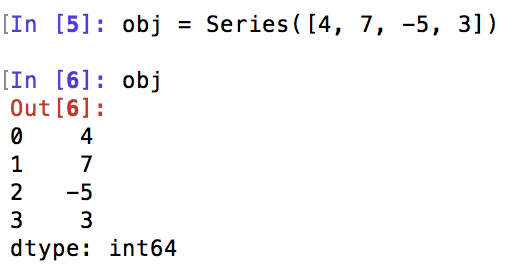
\includegraphics[width=.5\textwidth]{Cap4/imagens/pandas-series}}
	\caption{\textsc{Exemplo de uma \textit{Series}}}
	\vspace{-0.3cm}
	\legend{\small{FONTE: \citeonline{python-analysis}}}
	\label{pandas-series}
\end{figure}

\textit{DataFrame} representa uma tabela, uma estrutura de dados do tipo planilha, que possui uma coleção ordenada de colunas, onde cada uma delas pode ter um tipo de valor diferente (numérico, \textit{string}, \textit{boolean}, etc.). O \textit{DataFrame} possui um índice para linhas e também para colunas. Pode ser interpretado como um dicionário de \textit{Series}. De uma maneira geral, o dado é armazenado como um ou mais blocos bi-dimensionais ao invés de uma lista, dicionário, ou outro tipo de coleção de matriz unidimensional \cite{python-analysis}.

Existem várias maneiras diferentes de se criar um \textit{DataFrame}, entretanto uma forma comum é um dicionário de dimensões iguais, conforme a Figura~\ref{pandas-dataframe} e Figura~\ref{pandas-dataframe2},  ou uma matriz \textit{NumPy}.

\begin{figure}[h!]
	\centering
	\fbox{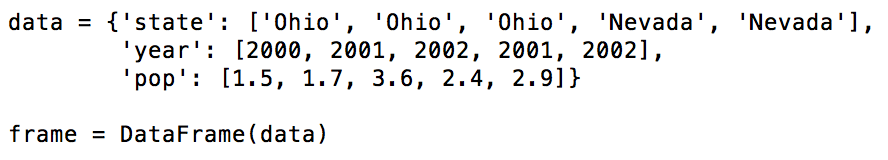
\includegraphics[width=.9\textwidth]{Cap4/imagens/pandas-dataframe}}
	\caption{\textsc{Criação de um \textit{DataFrame}}}
	\vspace{-0.3cm}
	\legend{\small{FONTE: \citeonline{python-analysis}}}
	\label{pandas-dataframe}
\end{figure}

\begin{figure}[h!]
	\centering
    \fbox{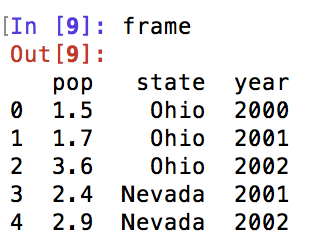
\includegraphics[width=.36\textwidth]{Cap4/imagens/pandas-dataframe2}}
	\caption{\textsc{Conteúdo de um \textit{DataFrame} pelo interpretador \textit{IPython}}}
	\vspace{-0.3cm}
	\legend{\small{FONTE: \citeonline{python-analysis}}}
	\label{pandas-dataframe2}
\end{figure}

%%% sub: matplotlib
\subsubsection{\textbf{\textit{matplotlib}}}
\textit{matplotlib} é uma biblioteca desenvolvida para a geração de gráficos bidimensionais a partir de \textit{arrays}. Gráficos comuns podem ser criados com alta qualidade a partir de simples comandos, inspirados nos comandos gráficos do MATLAB, exemplo ilustrado na Figura~\ref{matplotlib-fig}.

Quando usado em conjunto com ferramentas GUI (\textit{IPython}, por exemplo), esta biblioteca possui recursos interativos como zoom e visão panorâmica. \textit{matplotlib} suporta várias ferramentas GUI \textit{backend}, nos diversos sistemas operacionais suportados pelo Python, e permitem exportar gráficos em diversos formatos: PDF, SVG, JPG, PNG, BMP, GIF, etc.

\textit{matplotlib} também possui várias ferramentas adicionais, como o \textit{mplot3d} para plotar gráficos em tridimensionais e \textit{basemap} para mapeamentos e projeções.

\begin{figure}[h!]
  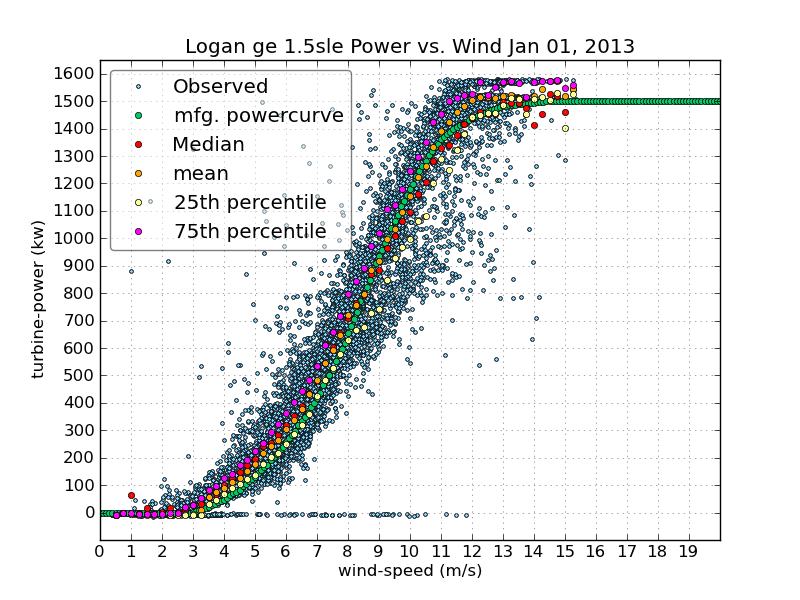
\includegraphics[width=1\textwidth]{Cap4/imagens/matplotlib}
  \caption{\textsc{Exemplo de um gráfico gerado pelo \textit{matplotlib}}}
  \vspace{-0.3cm}
  \legend{\small{FONTE: \citeonline{matplotlib}}}
  \label{matplotlib-fig}
\end{figure}


%%% sub: SciPy
\subsubsection{\textbf{\textit{SciPy}}}
\textit{SciPy} é uma coleção de pacotes que abordam uma série de soluções para diferentes domínios na computação científica. Na lista a seguir são apresentados exemplos desses pacotes \cite{python-analysis}:

\begin{itemize}
	\item \textit{scipy.integrate}: rotinas de integração numéricas e soluções de equações diferenciais;
	\item \textit{scipy.linalg}: rotinas de álgebra linear e decomposição de matrizes;
	\item \textit{scipy.optimize}: funções otimizadoras (minimizadoras) e algoritmos de busca em raíz;
	\item \textit{scipy.signal}: ferramentas para processamento de sinais;
	\item \textit{scipy.sparse}: matrizes esparsas e soluções de sistemas lineares esparsos;
	\item \textit{scipy.special}: agregador do \textit{SPECFUN}, uma biblioteca do Fortran que implementa várias funções matemáticas, como exemplo, a função gama;
	\item \textit{scipy.stats}: funções estatísticas, variáveis contínuas e discretas, testes estatísticos e outros modelos estatísticos;
	\item \textit{scipy.weave}: ferramenta para usar códigos \textit{inline} de C++ para acelerar a computação de matrizes.
\end{itemize}


%%% sub: IPython
\subsubsection{\textbf{\textit{IPython}}}
\textit{IPython} foi desenvolvido com o intuito de ser um interpretador interativo para o Python que teve início em 2001. Desde a sua criação o \textit{IPython} evoluiu grandemente, ao ponto de ser considerada uma das mais importantes ferramentas para computação científica em Python. Essa biblioteca não oferece nenhuma ferramenta para análise de dados ou análise computacional em si, sendo designada para maximizar a produtivadade tanto na interação computacional como no desenvolvimento de softwares. Oferece um fluxo de visualização de um modo \textit{execute-explore} ao invés do típico modelo \textit{edit-compile-run} de muitas outras linguagens de programação. Ela também provê uma pequena integração com o \textit{shell} e o sistema de arquivos de sistema operacional. Como a maior parte da programação focada na mineração de dados envolve exploração, tentativa e erro, e iteração, \textit{IPython}, em quase todos os casos, irá facilitar este tipo de trabalho \cite{python-analysis}.

Hoje, o projeto \textit{IPython} engloba muito mais do que apenas um interpretador \textit{shell} para Python. Ele também inclui um console gráfico interativo, o \textit{IPython Notebook}, que provê ao usuário uma experiência de caderno (\textit{notebook-like}) através de um navegador \textit{web}, conforme Figura~\ref{ipython-fig}, e dispõe de um mecanismo de processamento paralelo. Assim como muitas outras ferramentas desenvolvidas para programadores, é extremamente customizável \cite{mining-social-web}. \\ \\ \\ \\ \\ \\ \\

\begin{figure}[h!]
  \centering
  \fbox{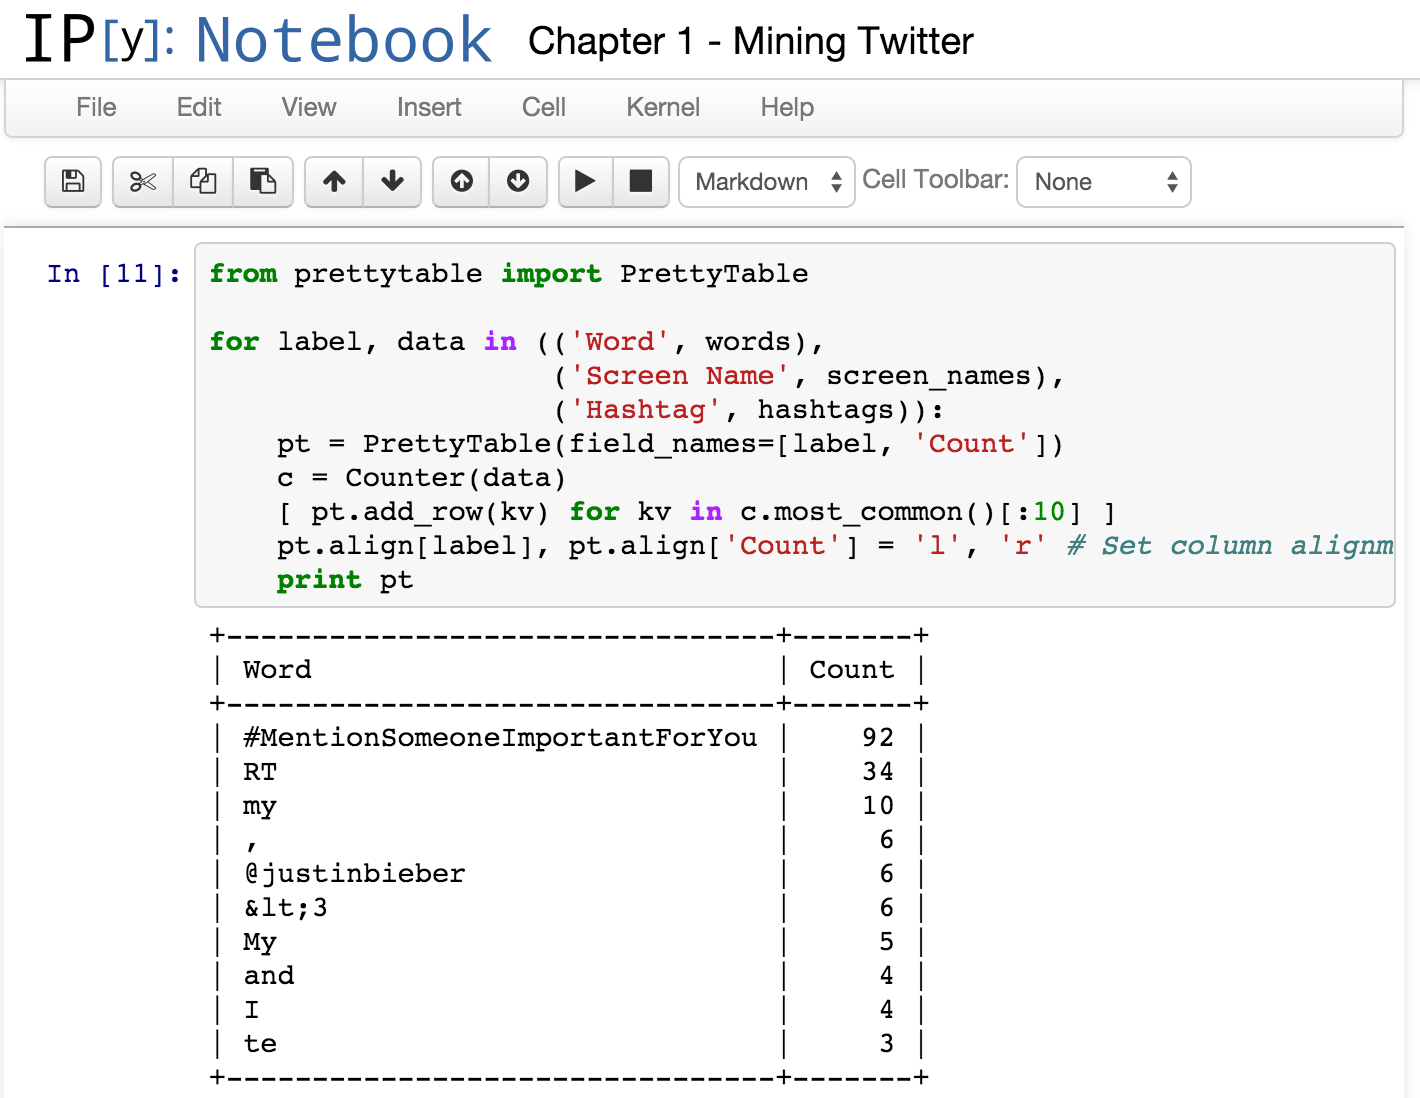
\includegraphics[width=0.9\textwidth]{Cap4/imagens/ipython-notebook}}
  \caption{\textsc{Exemplo de uma página \textit{web} do \textit{IPython Notebook}}}
  \vspace{-0.3cm}
  \legend{\small{FONTE: \citeonline{python-analysis}}}
  \label{ipython-fig}
\end{figure}

% python-linkedin
\subsubsection{\textbf{\textit{python-linkedin}}}
Esta biblioteca provê ao Python a API do \textit{LinkedIn}. Através da utilização do protocolo OAuth 2.0, é possível acessar diveros campos como \textit{Profile}, \textit{Group}, \textit{Company}, \textit{Jobs}, \textit{Search}, \textit{Share}, \textit{Network} e requisições REST APIs \cite{python-linkedin}.

%%
% API
\subsection{Interface de Programação de Aplicações - API}\label{subsec: api}
API é uma sigla para \textit{Application Programming Interface} e basicamente é uma tecnologia que permite um pedaço de \textit{software} se comunicar com outro pedaço de \textit{software}. Existem vários tipos de API e é comumente referenciado a outras tecnologias. Por exemplo para o desenvolvimento deste trabalho será utilizado a API do \textit{LinkedIn}. 

Uma API é composta por uma série de funções acessíveis somente por programação, e que permitem utilizar características do \textit{software} menos evidentes ao utilizador tradicional.


%% 
% REST API
\subsubsection{\textbf{Arquitetura REST}}
REST foi um termo criado por \citeonline{rest}, onde ele modela um estilo de arquitetura para a construção de serviços \textit{web} consistentes e coesos. O estilo da arquitetura REST é baseado em recursos e nos estados desses recursos.

Abreviação para Transferência de Estado Representacional, REST, é um estilo arquitetural baseado em recursos e nas representações desses recursos. Enfatiza a escalabilidade na interação entre componentes, a generalidade de interfaces, a implantação independente dos componentes de um sistema, o uso de componentes intermediários visando a redução na latência de interações, o reforço na segurança e o encapsulamento de sistemas legados. O REST ignora os detalhes da implementação de componente e a sintaxe de protocolo com o objetivo de focar nos papéis dos componentes, nas restrições sobre sua interação com outros componentes e na sua interpretação de elementos de dados significantes \cite{rest}.

A funcionalidade de uma REST API é similar ao funcionamento de uma página \textit{web}, onde o usuário efetua uma requisição a um servidor \textit{web}, utilizando o protocolo HTTP, e recebe dados como resposta.

Um recurso é qualquer conteúdo ou informação que é exposto na Internet, podendo ser um documento, vídeo clip, até processos de negócio ou dispositivos. Para utilizar um recurso é necessário ser capaz de identificá-lo na rede e de ter meios para manipulá-lo. Tem-se então o \textit{Uniform Resource Identifiers} (URI) para este propósito. Um URI unicamente identifica um recurso e, ao mesmo tempo, torna ele endereçável ou capaz de ser manipulado utilizando um protocolo, como o HTTP. O URI de um recurso se distingue dos de qualquer outro recurso e é através do próprio URI que ocorrem as interações com o recurso \cite{rest-book}.

Recursos devem possuir pelo menos um identificador para ser endereçável, e cada identificador é associado com uma ou mais representações. Uma representação é uma transformação ou uma visão do estado do recurso em um instante de tempo. Essa visão é codificada em um ou mais formatos transferíveis, tal como XHTML, Atom, texto simples, XML, YML, JSON, JPG, MP3, entre outros  \cite{rest-book}.

Os recursos provêm o conteúdo ou objeto com o qual se quer interagir e para atuar sobre eles é utilizado os métodos de HTTP. Os métodos HTTP na arquitetura REST podem ser referenciados como Verbos, uma vez que representam ações sobre os recursos \cite{rest-book}.


\subsection{Protocolo de Autenticação - OAuth}
Protocolos de autenticação são capazes de simplesmente autenticar a parte que está se conectando, ou ainda de autenticar a parte que está conectando assim como se autenticar para ele.

Neste trabalho será utilizado apenas o protocolo OAuth 2.0 para o acesso aos dados do \textit{LinkedIn}. É possível também realizar a autenticação utilizando a versão mais antiga, OAuth 1.0a, mas será apenas referenciado, neste trabalho, para a melhor compreensão do funcionamento do protocolo.

OAuth é uma sigla para "\textit{open authorization}", ou autorização aberta, e provê um meio para que usuários autorizem uma aplicação acessar dados, com alguma finalidade, através de uma API sem que os usuários precisem passar credenciais como nome de usuário e senha. De um modo geral, usuários são capazes de controlar o nível de acesso para estas aplicações e revogar este controle a qualquer momento \cite{mining-social-web}.

\subsubsection{\textbf{OAuth 1.0a}}
OAuth 1.0a é um protocolo que permite que um cliente (\textit{client}) \textit{web} tenha acesso a um recurso protegido pelo seu dono em um servidor. Esta definição se dá através da RFC 5849. Que são documentos técnicos desenvolvidos e mantidos pelo Internet Enginnering Task Force (IETF), instituição que especifica os padrões que serão implementados e utilizados em toda a Internet.

A razão para a existência dessa tecnologia é para evitar problemas de usuários (donos dos recursos) compartilhar suas senhas com aplicações \textit{web}.

A versão OAuth 1.0a não permite que credenciais sejam trocadas utilizando uma conexão \textit{Secure Socket Layer} (SSL) através de um protocolo HTTPS, por esse motivo muitos desenvolvedores achavam tedioso o trabalho devido aos vários detalhes envolvidos em encriptação.

SSL é um padrão global para tecnologia de segurança. Tem como função principal criar um canal criptografado entre um servidor \textit{web} e um navegador (\textit{browser}) para garantir que todos os dados transmitidos sejam seguros e sigilosos.

Uma aplicação que está requerindo acesso é conhecida como \textit{client}, em alguns momentos chamado de \textit{consumer}, a rede social ou o serviço que contém os recursos protegidas é nomeado como \textit{server} (também chamado de \textit{provider}) e o usuário que concede o acesso é o \textit{resource owner} (dono do recurso, tradução livre). Com estes elementos, três participações envolvem o processo e a interação que estes elementos possuem é conhecida como \textit{"three-legged-flow"} ou de uma maneira mais coloquial, a \textit{OAuth dance}. Estas são as etapas fundamentais que envolvem a \textit{OAuth dance} que, como resultado, permite ao \textit{client} o acesso a recursos protegidos, conforme listado a seguir \cite{mining-social-web}:

\begin{enumerate}
	\item O \textit{client} obtêm um \textit{token} de requisição do servidor de serviço (aplicação);
	\item O dono do recurso autoriza o \textit{token} de requisição;
	\item O \textit{client} troca o \textit{token} de requisição por um \textit{token} de acesso;
	\item O \textit{client} usa o \textit{token} de acesso para acessar os recursos protegidos com a consideração do dono do recurso.
\end{enumerate}

Para credenciais particulares, um \textit{client} começa com um uma \textit{consumer key} e um \textit{consumer secret} e no fim do processo de \textit{OAuth dance} termina com um \textit{token} de acesso e \textit{token} de acesso secreto que pode ser usado para acessar recursos protegidos.

\subsubsection{\textbf{OAuth 2.0}}
Enquanto o protocolo OAuth 1.0a permite uma autorização útil para o acesso a aplicações \textit{web}, OAuth 2.0 foi originalmente destinado a simplificar significantemente a implementação detalhada para desenvolvedores de aplicações \textit{web}, baseando-se completamente no SSL para aspectos de segurança e satisfazer uma vasta quantidade de casos de uso. Esses casos de uso variaram desde suporte para dispositivos móveis à necessidades empresariais e, consequentemente as necessidades de um termo mais futuro, da "Internet das Coisas"\space \cite{mining-social-web}.

Diferentemente da implementação OAuth 1.0a, que consiste de um rígido conjunto de etapas, a implementação do OAuth 2.0, definido através do RFC 6749, pode variar de acordo com a particularidade do caso de uso. Um decorrer típico da execução do OAuth 2.0 tem a vantagem do SSL e essencialmente contém apenas poucos redirecionamentos que, acompanhada de em alto-nível, não possui tanta diferença em relação ao processo anterior que envolvem um ciclo do OAuth 1.0a.

%%
% Linkedin
\subsection{LinkedIn}
\textit{LinkedIn} é uma rede social diferenciada, pois é voltada para perfis profissionais. Os usuários geralmente utilizam a rede como um currículo \textit{online}, procuram se relacionar com novos contatos para aumentar a sua rede de conhecimentos profissionais e também para encontrar e conhecer novas oportunidades tanto de ocupação quanto de negócio.

A mineração de dados através da rede \textit{LinkedIn} se dá utilizando a API que ela dispõe. Para isso é necessário possuir uma conta na rede social.

A grande parte das análise realizadas neste projeto acontece utilizando arquivos \textit{comma-separated values} (CSV), que é possível baixá-lo.

Na Subseção~\ref{api-linkedin} é apresentado a API do \textit{LinkedIn} e como se obter dados através dela.

\subsubsection{\textbf{API LinkedIn}}\label{api-linkedin}
O acesso a API se dá através da criação de uma aplicação pela página \textit{web} de desenvolvimento do \textit{LinkedIn}. Após a criação da aplicação é fornecido ao usuário informações para o acesso utilizando o protocolo OAuth, será informado uma chave da API da aplicação, uma chave secreta, o \textit{token} de usuário OAuth e credenciais secretas do usuário OAuth.

Dispondo de todas as credenciais do protocolo OAuth o acesso a API acontece utilizando a biblioteca \textit{python-linkedin}, especificada na Subseção~\ref{sec:bib_python}.

Os dados disponibilizados pela API está limitado basicamente ao o que o usuário consegue usufruir da experiência através da página \textit{web}. Restrições como a visualização de "amigos de amigos" \space também existem, demonstrando ser uma API um tanto restrita. Essa restrição é proposital e importante para a política do \textit{LinkedIn}. Portanto é possível fazer buscas de pessoas, companhias, empregos, conexões, grupos e outros elementos que a API disponibiliza \cite{mining-social-web}.

Conforme descrito anteriormente, é possível fazer o \textit{download} dos dados, visíveis ao usuário, em formato CSV. Podendo ser especificados em títulos de trabalho ou contatos através de uma opção de exportação presente no menu da página do \textit{LinkedIn}.

%%
% METODOLOGIA
\section{METODOLOGIA E DESENVOLVIMENTO}\label{sec: metodologia}
O processo de desenvolvimento da solução segue uma série de princípios de conjunto de boas práticas e etapas do \textit{data mining}, para melhor estruturar e obter, não só o resultado esperado, mas também para que todo o processo ocorra de forma coerente e padronizada.

%%
% Etapas do Data Mining
\subsection{Etapas Para a Mineração de Dados do \textit{LinkedIn}}
Abordado previamente, o acesso aos dados do \textit{LinkedIn} acontece através da utilização de sua API. A análise necessária para a interpretação dos dados se dá pela aplicação da técnica de \textit{clustering}, normalização de dados e computação de similaridade. 

\subsubsection{\textbf{\textit{Clustering}}} 
Um aprendizado não supervisionado que está presente em várias ferramentas de \textit{data mining}. A técnica de \textit{clustering} envolve em pegar uma coleção de itens e particioná-los em pequenas coleções, conhecidos como \textit{cluster}, de acordo com alguma heurística que será usado para comparar com outros itens da coleção.

Técnicas para \textit{clustering} são partes fundamentais para um processo de mineração de dados. Uma implementação simples de \textit{clustering} pode criar experiências de usuário incrivelmente convincentes para alcançar resultados. Também pode ser aplicado a bases de texto utilizando algoritmos de \textit{text mining}, onde o algoritmo procura agrupar textos que falem sobre o mesmo assunto e separar textos de conteúdo diferentes.

Por exemplo, caso queira considerar a localização geográfica dos contatos na rede \textit{LinkedIn}, é necessário realizar um \textit{cluster} nas conexões através de um determinado número de regiões com o intuito da melhor compreensão de oportunidades econômicas disponíveis.

\subsubsection{\textbf{Normalização de Dados}}
Quando se recupera dados provenientes de uma API, é muito comum que esses não estarão no formato desejado para a sua análise. No caso do \textit{LinkedIn}, pode ser que usuários procurem por vagas de emprego escrevendo os nomes das vagas de alguma outra maneira sem ser o nome correto da vaga. Como exemplo, uma vaga para administrador de banco de dados pode ser buscado através da sigla "DBA", que em inglês significa \textit{Database Administrator}.

A normalização de dados, procura então resolver esses problemas padronizando situações específicas que irá facilitar a análise posterior dos dados.

\subsubsection{\textbf{Computação de Similaridade}}
Após a normalização dos itens, é preciso verificar a similaridade entre eles. Podendo ser vagas de emprego, nomes de empresas, interesses profissionais, indicação geográfica, ou qualquer outro campo digitado na busca como um texto livre. Para isso é necessário definir uma heurística que conseguirá aproximar a similaridade entre dois valores quaisquer. Em algumas situações a similaridade heurística será um tanto óbvia, porém em outros casos será complicada. Por exemplo, comparar o tempo de carreira entre duas pessoas pode ser simples como uma operação de soma ou subtração. Mas comparar um elemento profissional, como "atitude de liderança" \space de uma maneira automatizada pode ser um desafio.

\section{CONSIDERAÇÕES FINAIS}
A utilização das bibliotecas que Python oferece para a mineração de dados permite que o desenvolvimento das soluções se tornem mais rápidos e efetivos. Assim como a utilização da API do \textit{LinkedIn} para a obtenção dos dados e as etapas do processo de \textit{data mining}. Boas práticas, protocolos e tecnologias são aproveitadas no andamento deste trabalho. Considerando os conceitos até aqui abordados, é possível compreender de forma clara os tópicos seguintes.























%\bookmarksetup{startatroot}

% ----------------------------------------------------------
% ELEMENTOS PÓS-TEXTUAIS
% ----------------------------------------------------------
\postextual

\bibliography{Configuracoes/citacoes} % Referências bibliográficas

%\begin{apendicesenv}% Apêndices: inserir se necessário
%\partapendices
%  \input{Extras/apendice1}
%  \input{Extras/apendice2}
%\end{apendicesenv}

%\begin{anexosenv}% Anexos: inserir se necessário
%\partanexos
% \input{Extras/anexo1}
% \input{Extras/anexo2}
% \input{Extras/anexo3}
%\end{anexosenv}

\printindex % Indice Remissivo
\end{document}
